\documentclass{article}
\usepackage{graphicx}
\usepackage{amsmath}
\usepackage{pgfplots}

\begin{document}
\title{Maths Assignment}
\author{Karyampudi Meghana Sai\\ EE23BTECH11031}
\maketitle

\section*{Problem Statement}
Write the first five terms of the sequence \(a_n = \frac{n(n^2+5)}{4}\).

\section*{Solution}


The relation between x(n) and u(n):
\begin{align}
 x(n) = \left(\frac{(n+1)^3+5(n+1)}{4}\right) u(n)
 \end{align}
Z-transform of $n^ku(k)$ in terms of kth derivative of U(z):
\begin{align}
n^k u(n) &\overset{\text{ZT}}{\longleftrightarrow} (-1)^k z^k \frac{d^k}{dz^k}U(z)
\end{align}
The Z-transform of $nu(n)$ is given by:
\begin{align}
\mathcal{Z}\{nu(n)\} &= \frac{z^{-1}}{(1 - z^{-1})^2}
\end{align}
\text{ROC :} $\lvert z \rvert > 1$\\
The Z-transform of $n^2u(n)$ is given by:
\begin{align}
\mathcal{Z}\{n^2u(n)\} &= \frac{(z^{-1})(1+z^{-1})}{(1-z^{-1})^3}
\end{align}
\text{ROC :} $\lvert z \rvert > 1$\\
The Z-transform of $n^3u(n)$ is given by:
\begin{align}
\mathcal{Z}\{n^3u(n)\} &= \frac{(z^{-1})(1+4z^{-1}+z^{-2})}{(1-z^{-1})^4}
\end{align}
\text{ROC :} $\lvert z \rvert > 1$\\
Now Z-transform of x(n) is given by:
\begin{align}
\mathcal{Z}\{x(n)\} &=\frac{\mathcal{Z}\{n^3u(n)\}}{4} +\frac{3\mathcal{Z}\{n^2u(n)\}}{4} +2\mathcal{Z}\{nu(n)\} +\frac{3\mathcal{Z}\{u(n)\}}{2}\\
\mathcal{Z}\{x(n)\} &=\frac{(z^{-1})(1+4z^{-1}+z^{-2})}{4(1-z^{-1})^4} +\frac{3(z^{-1})(1+z^{-1})}{4(1-z^{-1})^3} +\frac{2z^{-1}}{(1 - z^{-1})^2} +\frac{3}{2(1- z^{-1})}
\end{align}
\newpage
\begin{figure}
    \centering
    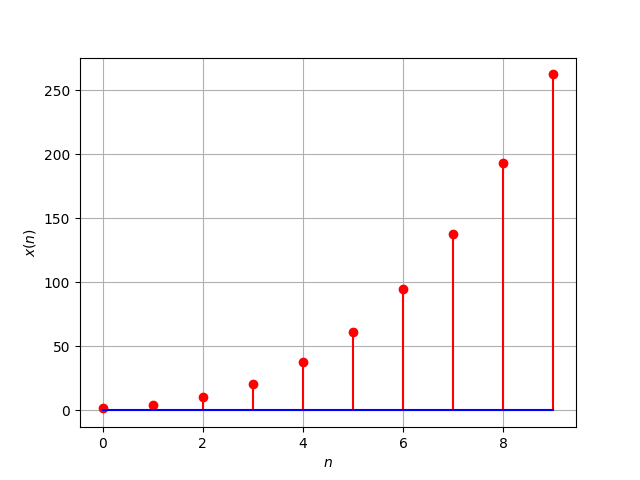
\includegraphics{figs/plot.png}
    \caption{Plot of equation(1)}
    \label{fig:plot}
\end{figure}


\end{document}

